% Appendix A

\chapter{Code Examples} % Main appendix title

\label{AppendixA} % For referencing this appendix elsewhere, use \ref{AppendixA}

\section{MPI Operations}

The color of links can be changed to your liking using:
%
%{\small\verb!\hypersetup{urlcolor=red}!}, or
%
%{\small\verb!\hypersetup{citecolor=green}!}, or
%
%{\small\verb!\hypersetup{allcolor=blue}!}.
%
%\noindent If you want to completely hide the links, you can use:
%
%{\small\verb!\hypersetup{allcolors=.}!}, or even better: 
%
%{\small\verb!\hypersetup{hidelinks}!}.
%
%\noindent If you want to have obvious links in the PDF but not the printed text, use:
%
%{\small\verb!\hypersetup{colorlinks=false}!}.

\subsection {Broadcast Example}
\label{appendix:broadcast}
\begin{verbatim}

from mpi4py import MPI
comm = MPI.COMM_WORLD
rank = comm.Get_rank()

if rank == 0:
	data = {'key1' : [7, 2.72, 2+3j],'key2' : ( 'abc', 'xyz')}
	print 'Broadcasting...',data
else:
	data = None
	
data = comm.bcast(data, root=0)
print 'Broadcasting...',data

\end{verbatim}

\bf{Output:}
\begin{center}
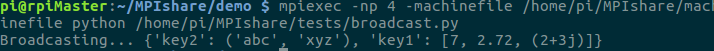
\includegraphics[scale=0.7]{Figures/broadcast-output}
\end{center}

\subsection {Scatter Example}
\label{appendix:scatter}
\begin{verbatim}
from mpi4py import MPI
comm = MPI.COMM_WORLD
size = comm.Get_size()
rank = comm.Get_rank()

if rank == 0:
	data = [(i+1)**2 for i in range(size)]
else:
	data = None

data = comm.scatter(data, root=0)
assert data == (rank+1)**2

\end{verbatim}

\bf{Output:}
\begin{center}
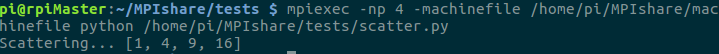
\includegraphics[scale=0.7]{Figures/scatter-output}
\end{center}

\begin{verbatim}

\end{verbatim}

\subsection {Gather Example}
\label{appendix:gather}

\begin{verbatim}
from mpi4py import MPI

comm = MPI.COMM_WORLD
size = comm.Get_size()
rank = comm.Get_rank()

data = (rank+1)**2
data = comm.gather(data, root=0)

if rank == 0:
	for i in range(size):
		assert data[i] == (i+1)**2
		print data[i],'from node',i
	print 'The final array:',data
else:
	assert data is None



\end{verbatim}

\bf{Output:}
\begin{center}
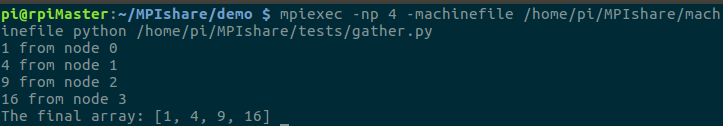
\includegraphics[scale=0.7]{Figures/gather-output}
\end{center}

\begin{verbatim}

\end{verbatim}

\subsection {Reduction Example}

\label{appendix:reduction}
\begin{verbatim}
from mpi4py import MPI
import numpy
import sys
comm = MPI.COMM_SELF.Spawn(sys.executable,args=['cpi.py'],maxprocs=5)
N = numpy.array(100, 'i')
comm.Bcast([N, MPI.INT], root=MPI.ROOT)
PI = numpy.array(0.0, 'd')
comm.Reduce(None, [PI, MPI.DOUBLE],op=MPI.SUM, root=MPI.ROOT)
print (PI)
comm.Disconnect()
\end{verbatim}

\bf{Output:}
\begin{center}
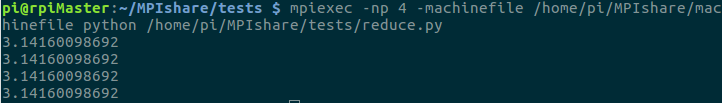
\includegraphics[scale=0.7]{Figures/reduce-output}
\end{center}

\begin{verbatim}

\end{verbatim}